\chapter{Erstellung des softaware/webdev-Docker-Containers}
\label{cha:implementation}
In diesem Abschnitt wird beschrieben, aus welchen Bestandteilen der Container besteht, warum diese Entscheidungen getroffen wurden und welche Probleme und Hürden sich bei der Entwicklung ergaben.
Weiters wird dargestellt, in welchen Aspekten der Container durch neue Kenntnisse beim Einsatz in echten Projekten weiterentwickelt wurde.

\section{Anwendungsszenarien}

run npm
add as dependency
inherit

\begin{lstlisting}[caption=Kommando zum Starten des softaware/webdev-Containers, language=bash, label=lst:docker-run-webdev]
docker run -it --rm -v ${pwd}:/usr/app/src softaware/webdev:alpine-8.1.2
\end{lstlisting}

\begin{figure}[htbp]
    \centering
    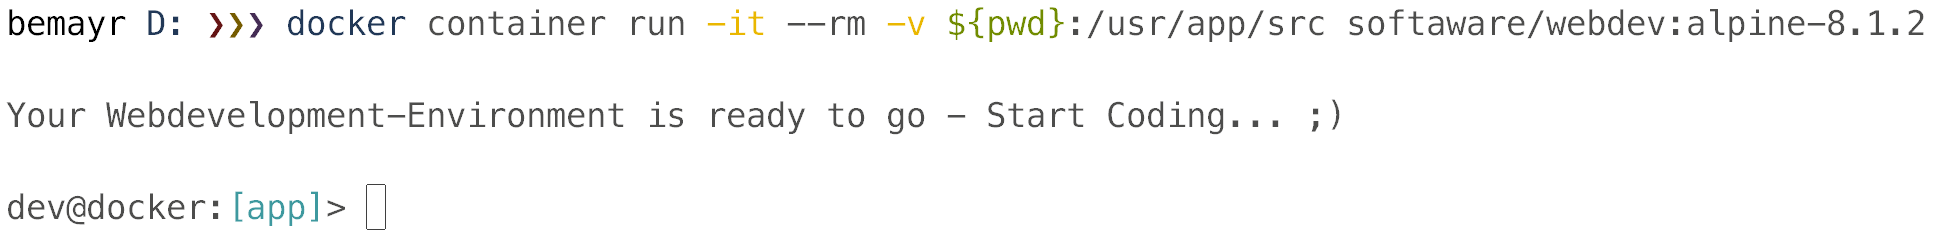
\includegraphics[width=0.92\linewidth,clip]{images/container-execution}
    \caption{Ausgabe beim Start des Containers}
\label{fig:container-execution}
\end{figure}

\section{Dockerfile}
\label{sec:dockerfile}
\lstinputlisting[caption=Alpine-Dockerfile,label={lst:dockerfile.alpine}]{listings/Dockerfile.alpine}

\lstinputlisting[caption=Bash-Konfigurationsdatei,label={lst:.bashrc},language=bash]{listings/.bashrc}

https://tex.stackexchange.com/questions/144170/lstlistings-reference-to-line-number
https://tex.stackexchange.com/questions/116216/is-there-a-possibility-to-make-reference-to-the-line-in-the-lstlisting-environme

Volumes
. Node modules Typescript
. Port mappings + Geschichte des Containers

https://docs.npmjs.com/cli/completion

run command
https://serverfault.com/questions/685697/multiple-commands-in-docker-cmd-directive
% https://docs.docker.com/engine/reference/builder/#cmd

\subsubsection{Zeile 2}
Die \verb|FROM|-Anweisung ermöglicht es Docker-Images voneinander zu erben.
In diesem Fall wird vom offiziellen node-Image\footnote{\url{https://hub.docker.com/_/node/}} geerbt.
Dieses beinhaltet Node.js, npm und yarn, wodurch die gesamte Basisfunktionalität bereits vorhanden ist.

\verb|{{ node_version }}| ist keine Funktionalität von Docker, dies ist ein Platzhalter für die Versionsnummer des Node.js-Images im Build-Prozess (vgl. \cref{sec:build-process}).
Der Name des offiziellen Node.js-Images beginnt mit der Node.js-Versionsnummer und enthält die Art des Images als Suffix.
In diesem Fall wird von dem \emph{alpine}-Image abgeleitet und der Platzhalter im Build-Prozess durch die konkrete Versionsnummer ersetzt.

\subsubsection{Zeile 3}
Die früher verwendete \verb|MAINTAINER|-Anweisung in Dockerfiles wurde durch das flexiblere \verb|LABEL| ersetzt.
Durch den \emph{maintainer} werden Metadaten erstellt, die angeben wer für dieses Image verantwortlich ist, und an wen sich der Benutzer dessen wenden kann.

\subsubsection{Zeile 6}
Wie im Kommentar in Zeile 5 beschrieben, wird durch die \verb|ENV|-Anweisung die Umgebungsvariable \verb|PATH| erweitert.
Diese Änderung ermöglicht es, lokal installierte Node.js-Anwendungen als Kommandos zu verwenden.

In \cref{sec:global-package-installation} wurde bereits der Unterschied zwischen global und lokal installierten Anwendungen erläutert.
Im Container ist allerdings aufgrund der Isolierung das in \autocite{stackoverflow:nodemodules-hack:online} beschriebene Sicherheitsrisiko wesentlich geringer.
Anstatt der Erstellung eines eigenen Container-Images mit global installierten Paketen, sollten diese bei der Verwendung des Containers immer in der \emph{package.json}-Datei erfasst werden.
Dadurch muss kein eigenes Image gewartet werden und auch ohne dem Container sind alle Abhängigkeiten des Webprojektes definiert.

Diese Änderung an der Umgebungsvariable ist lediglich aus Kompatibilitätsgründen vorhanden, damit auch ältere Projekte, die sich historisch bedingt auf globale Abhängigkeiten verlassen, im Container verwendet werden können.
Die Konfiguration eines Webprojektes sollte allerdings nach \cref{subsub:packages-best-practice} erfolgen.

\subsubsection{Zeile 9}
Hier wird unter der Verwendung des Alpine-Linux-Paketmanagers \emph{apk} die Bourne Again Shell installiert.
Im Gegensatz zur Almquist Shell ist sie wesentlich weiter verbreitet und bietet erweiterte Funktionalität.
Durch den \verb|--no-cache| Parameter wird die Größe des fertigen Docker-Images möglichst klein gehalten.

\subsubsection{Zeile 12}
In Zeile 12 wird das aktuelle Arbeitsverzeichnis des resultierenden Containers auf \verb|/usr/src/app| gesetzt.
Die \verb|WORKDIR|-Anweisung eines Dockerfiles entpricht im wesentlich dem Wechsel in dieses Verzeichnis mit \verb|cd|.

\subsubsection {Zeile 15}


\subsubsection {Zeile 16}
Beim Ausführen von Skripten, oder beispielsweise dem Deinstallieren von Paketen bietet npm auf der Kommandozeile die Möglichkeit der Autovervollständigung.
Diese wird aktiviert, indem das Kommando \verb|npm completion| ein Shell-Skript erstellt, das an die benutzerspezifische Shell-Konfiguration angehängt wird.

Das Ergebnis von \verb|npm completion| war in einer früheren Version des Containers bereits in \emph{.bashrc} integriert.
Falls dieses allerdings bei unterschiedlichen npm-Versionen unterschiedlich ausfällt, würde die Autovervollständigung nicht korrekt funktionieren.
Durch das nachträgliche Hinzufügen des Ergebnisses mithilfe der \verb|RUN|-Anweisung ist nun sichergestellt, dass das Ergebnis von \verb|npm completion| immer zur verwendeten npm-Version passt.

\subsubsection {Zeile 17}
shell form
überschrieben
bash
welcome message



\section{Build-Prozess}
\label{sec:build-process}
\lstinputlisting[caption=\emph{create-image.ps1} (Build-Skript des Containers),label={lst:create-image.ps1}]{listings/create-image.ps1}

\section{Alpine-Linux vs. Debian}
\label{sec:alpine-vs-debian}
\lstinputlisting[caption=Debian-Dockerfile,label={lst:dockerfile.debian}]{listings/Dockerfile.debian}

\section{Dokumentation}
\label{sec:documentation}

\subsection{Docker Hub}
\label{sub:dockerhub}
\subsection{Microbadger}
\label{sub:microbadger}
\subsection{Beispiele}
\label{sub:examples}


\section{Probleme}
\label{sec:container-problems}
different OSs -> delete node_modules
IDE automatic install
File Detection
